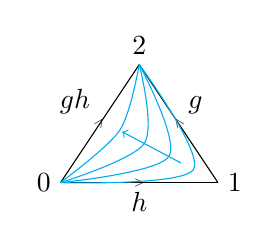
\begin{tikzpicture}
\node[above] (c) at (1,1.5) {$2$};
\node[left]  (a) at (0,0) {$0$};
\node[right] (b) at (2,0) {$1$};
\draw (0,0) -- (2,0)   node[sloped, scale=.5, pos=0.5] {$>$}
                       node[sloped, scale=1, pos=0.5, below] {$h$};
\draw (0,0) -- (1,1.5) node[sloped, scale=.5, pos=0.5] {$>$} 
                       node[scale=1, pos=0.5, above left] {$gh$};
\draw (2,0) -- (1,1.5) node[sloped, scale=.5, pos=0.5, xscale=-1] {$>$} 
                       node[scale=1, pos=0.5, above right] {$g$};

% a=.488, t=.2,.4,.6,.8: (2-(cos(a)*2)*t*cos(a), (cos(a)*2)*t*sin(a))
\draw [cyan] plot [smooth] coordinates { (0,0) (1.6879319857569757, 0.1656525284552739)  (1,1.5)};
\draw [cyan] plot [smooth] coordinates { (0,0) (1.3758639715139513, 0.3313050569105478)  (1,1.5)};
\draw [cyan] plot [smooth] coordinates { (0,0) (1.0637959572709272, 0.49695758536582163) (1,1.5)};
\draw [cyan] plot [smooth] coordinates { (0,0) (0.7517279430279029, 0.6626101138210956)  (1,1.5)};

% t=.3 to t=.78
\draw[cyan, -to] (1.5318979786354636, 0.24847879268291082) --
(0.7829347444522055, 0.6460448609755681);
\end{tikzpicture}
